\documentclass[a4paper]{article}

\usepackage[utf8x]{inputenc}
\usepackage{amsmath}
\usepackage{graphicx}
\usepackage{color}
\usepackage{listings}
\usepackage[T1]{fontenc}
\usepackage{lmodern}
\usepackage{amsthm}
\usepackage{amsfonts}
\usepackage{tikz}
\usepackage{placeins}
 
\tikzstyle{state}=[shape=circle,draw=blue!50,fill=blue!20]
\tikzstyle{observation}=[shape=rectangle,draw=orange!50,fill=orange!20]
\tikzstyle{lightedge}=[<-,dotted]
\tikzstyle{mainstate}=[state,thick]
\tikzstyle{mainedge}=[<-,thick]

\title{HMM digit recogniser}
\author{Soufian SALIM}

\lstset{ %
	language=R,
	basicstyle=\footnotesize,
	numbers=left,
	numberstyle=\footnotesize,
	stepnumber=1,
	numbersep=5pt,
	backgroundcolor=\color{white},
	showspaces=false,
	showstringspaces=false,
	showtabs=false,
	frame=single,
	tabsize=2,
	captionpos=b,
	breaklines=true,
	breakatwhitespace=false,
	escapeinside={\%*}{*)}
}

\begin{document}

\maketitle

\begin{abstract}

Report on the HMM digit recogniser project for the Signal et Langue course, ATAL master.

\end{abstract}

\newpage

\tableofcontents

\newpage

\section{Symbol sequence extraction}

\subsection{Extend the simu\_symbol function to simulate a third digit, select for instance a "6"}

\begin{lstlisting}
simu_symbol <- function() 
{
  (...)
  
  digit_6 <- rbind(
    stroke(0.25, 0.85, -0.4, -0.2, 10),
    stroke(-0.4, -0.2, 0, -1, 7),
    stroke(0, -1, 0.3, -0.5, 7),
    stroke(0.3, -0.5, -0.1, 0.3, 6)
  )
  
  dimnames(digit_6) <- list(num=1:nrow(digit_6), point=c("x", "y"))
  
  plot(digit_6, type="l", col="red", xlim=c(-1, 1), ylim=c(-1, 1))
  
  points(digit_6)
  
  return(list(d1=digit_1, d2=digit_4, d3=digit_6))
}
\end{lstlisting}

\subsection{Consider the [{\it compute\_symbol}] function to transform one digit in a sequence of symbols}

\textbf{Analyse this function and explain how it works.} \newline

The function takes the following as input: a digit trace, a number of rows ({\it nr}), and a number of columns ({\it nc}). It then takes the following steps: \newline

\begin{enumerate}

\item It creates a matrix of {\it nr} * {\it nc} dimensions, each box containing a number from 1 to 15, from the top left to the bottom right
\item It calculates the number of points in the inputted digit
\item It computes the horizontal position of each point
\item It computes the vertical position of each point
\item It computes, for each point, the corresponding box in the first matrix, and outputs it

\end{enumerate}

\textbf{Test it with the simulated digits.} \newline

In order, output for digit "1", digit "4" then digit "6":

\begin{lstlisting}
[1] 11 11 14 14 14 14 14 14 14 14 14 14 14 14 11 11 11 11  8  8  8  8  5  5  5  5  2  2  2  2
[1] 14 14 14 11 11 10  7  7  7  4  4  4  4  4  5  8  8  8  9  9  8  8  8  5  5  5  2  2  2  2
[1] 14 14 14 11 11 11  8  8  8  7  7  5  5  2  2  2  2  2  2  2  2  2  5  5  5  5  8  8  8 11
\end{lstlisting}

\textbf{From your point of view what are the strengths and weaknesses of this method.} \newline

This method allows for efficient resampling of a graphical digit (or other character). With enough rows and columns, it could technically differenciate between a digit and and exponent, or any other form of mathematical notation. \newline

Another advantage of this method is that the number of columns and rows does not affect the length of the outputted sequence, which is solely dependent on the number of points in the digit trace.  \newline

Its weakness, however, is that it can only be used for "online" writing (or would require strong preprocessing), since the order of each point is critical to the sequence construction.

\subsection{Now let us consider [{\it compute\_symbol\_dir}] to transform one digit in a sequence of symbols}

\textbf{Analyse this function and explain how it works.} \newline

The function takes the following as input: a digit trace, and a number of angle classes ({\it nangles}). It then computes the angle of a segment between two points, and classify it in one of {\it nangles} angle classes.  \newline

\textbf{Test it with the simulated digits.} \newline

In order, output for digit "1", digit "4" then digit "6":

\begin{lstlisting}
[1] "1:"
 1  2  3  4  5  6  7  8  9 10 11 12 13 14 15 16 17 18 19 20 21 22 23 24 25 26 27 28 29 30 
 2  2  2  2  2  2  2  2  2  7  7  7  7  7  7  7  7  7  7  7  7  7  7  7  7  7  7  7  7  7 
[1] "4:"
 1  2  3  4  5  6  7  8  9 10 11 12 13 14 15 16 17 18 19 20 21 22 23 24 25 26 27 28 29 30 
 6  6  6  6  6  6  6  6  6  5  1  1  1  1  1  1  1  1  1  4  7  7  7  7  7  7  7  7  7  7 
[1] "6:"
 1  2  3  4  5  6  7  8  9 10 11 12 13 14 15 16 17 18 19 20 21 22 23 24 25 26 27 28 29 30 
 6  6  6  6  6  6  6  6  6  1  8  8  8  8  8  8  1  2  2  2  2  2  2  1  4  4  4  4  4  4 
\end{lstlisting}

\textbf{From your point of view what are the strengths and weaknesses of this method.} \newline

Like with the previous method, one of the advantages is that the length of the sequence is not affected by the number of angle classes. Also like with the previous method, the order of each point is important and it cannot be used if the correct order is unknown. \newline

Unlike the previous method, since this one uses angles to resample the digits, it might allow for more subtle distinction between symbols (for example, the "1" and the british-style handwritten "7": both might be in the same "boxes" after resampling with the first method, but this one will show an angular difference).

\section{Selection of a HMM topology and initial values}

\subsection{Give a graphical representation of this model}

\FloatBarrier

\begin{figure}[htbp]
	\begin{center}
		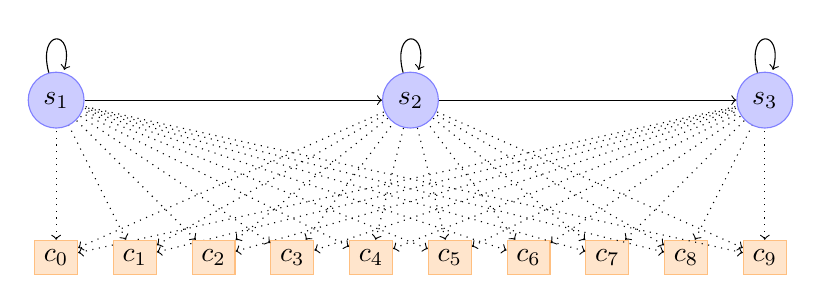
\begin{tikzpicture}[]

		% states
		\node[state] (s1) at (0,2) {$s_1$}
			edge [loop above] node[auto,swap] {} ();
		\node[state] (s2) at (4.5,2) {$s_2$}
			edge [<-,bend left=0] node[auto,swap] {} (s1)
			edge [loop above] node[auto,swap] {} ();
		\node[state] (s3) at (9,2) {$s_3$}
			edge [<-,bend left=0] node[auto,swap] {}  (s2)
			edge [loop above] node[auto,swap] {} ();
			
		% observations
		\node[observation] (y0) at (0,0) {$c_0$}
			edge [lightedge] (s1)
			edge [lightedge] (s2)
			edge [lightedge] (s3);
		\node[observation] (y1) at (1,0) {$c_1$}
			edge [lightedge] (s1)
			edge [lightedge] (s2)
			edge [lightedge] (s3);
		\node[observation] (y2) at (2,0) {$c_2$}
			edge [lightedge] (s1)
			edge [lightedge] (s2)
			edge [lightedge] (s3);
		\node[observation] (y3) at (3,0) {$c_3$}
			edge [lightedge] (s1)
			edge [lightedge] (s2)
			edge [lightedge] (s3);
		\node[observation] (y4) at (4,0) {$c_4$}
			edge [lightedge] (s1)
			edge [lightedge] (s2)
			edge [lightedge] (s3);
		\node[observation] (y5) at (5,0) {$c_5$}
			edge [lightedge] (s1)
			edge [lightedge] (s2)
			edge [lightedge] (s3);
		\node[observation] (y6) at (6,0) {$c_6$}
			edge [lightedge] (s1)
			edge [lightedge] (s2)
			edge [lightedge] (s3);
		\node[observation] (y7) at (7,0) {$c_7$}
			edge [lightedge] (s1)
			edge [lightedge] (s2)
			edge [lightedge] (s3);
		\node[observation] (y8) at (8,0) {$c_8$}
			edge [lightedge] (s1)
			edge [lightedge] (s2)
			edge [lightedge] (s3);
		\node[observation] (y9) at (9,0) {$c_9$}
			edge [lightedge] (s1)
			edge [lightedge] (s2)
			edge [lightedge] (s3);
			
		\end{tikzpicture}
	\end{center}
	
	\caption{An HMM with 3 states which can emit 10 symbols $c$. In this particular HMM, states can only reach themselves or the next state. Each state can emit any symbol.}
\end{figure}

\FloatBarrier

\subsection{How would you initialise the vector of initial probabilities, and the state transition matrix, knowing that the length of the sequences are T = 30?}

Initial probabilities: \newline

\begin{tabular}{ c | c | c }
  1 & 0 & 0 \\
\end{tabular}

\hspace{20mm}
\linebreak
Given that each state is in charge of generating one part of the digit, the first state models the beginning of the digit. Therefore the first state must always have an initial probability of 1, and the others of 0. \newline

State transition matrix: \newline

\begin{tabular}{ c | c | c | c }
  & s1 & s2 & s3 \\
  \hline
  s1 & 0.9 & 0.1 & 0.0 \\
  \hline
  s2 & 0.0 & 0.9 & 0.1\\
  \hline
  s3 & 0.0 & 0.0 & 1.0 \\
\end{tabular}

\hspace{20mm}
\linebreak
Since a sequence is of length T = 30, and there are three states, on average there should be 1 in 10 chances of moving to the next state and 9 in 10 of staying on the same state (length of sequence / number of state), because we want to stay on each state roughly the same amount of time. \newline

\subsection{How about the observation matrix?}

Without any more information on the digits we can only start with a uniform distribution for the observation matrix.

\section{Training of the models}

\subsection{Create a first function {\it initHMMDigit} which takes as input the number of states and of possible observations, and initialise the transition matrix with a left-right architecture and with uniform distribution of observations from each state}


\begin{lstlisting}
initHMMDigit <- function(nsymbols=15, nstates=3, uniform=F)
{
  states <- c(paste("Tier", 1:nstates))
  symbols <- 1:nsymbols
  startProbs <- c(1, c(rep(0, nstates-1)))
  
  if (uniform) distr <- c(0.5, 0.5) else  distr <- c(1 - nstates / 30, nstates / 30)
  
  transProbs <- matrix(c(
    rep(c(distr, rep(0.0, nstates-1)), nstates-1), 1.0
    ), nrow=nstates, ncol=nstates, byrow=T
  )
  
  emissionProbs <- matrix(
    rep(1/nsymbols, nsymbols * nstates),
    nrow=nstates, ncol=nsymbols, byrow=T
  )
  
  hmm <- initHMM(states, symbols, startProbs, transProbs, emissionProbs)
}
\end{lstlisting}

\subsection{Have a look at the different models after training. Do they make sense for you?}

Their probability to move on to the next state has slightly reduced, therefore limiting lightly the time spent on the last state. \newline

The emission probabilities are no longer uniformly distributed; altough not that significantly. \newline

\subsection{Select a specific model of digit, and consider the symbols that will be most often emitted during states 1, 2 and 3}

For the 1, for example, using a model trained on data generated with the first sampling method (3x5), we can see that emissions probabilities are higher for symbols 2, 5, 8, 11 and 14. These symbols correspond to the "middle boxes" in the sampling method.

\section{Recognition performances}

\subsection{Use the corresponding test files, and run the forward algorithm to build the confusion
matrix for these four cases, display the global recognition rates}

For the "3\_5" type, with 3 states, optimal distribution:\newline

\begin{tabular}{ c | c | c | c | c | c | c | c | c | c | c }
  0 & 1 & 2 & 3 & 4 & 5 & 6 & 7 & 8 & 9 \\
  \hline
  0 & \textbf{121} & 1 &  0 &  0 &  0 &  2  & 1 & 0 & 4 & 0 \\
  \hline
  1 & 1 & \textbf{104} & 23 &  0 &  1 &  0 &  0  & 3 & 1 & 3 \\
  \hline
  2 & 4 & 1 & \textbf{102}  & 1  & 8 &  0  & 4  & 2 & 1 & 15 \\
  \hline
  3 & 0 & 0 &  2 & \textbf{128} &  1 &  0  & 0  & 3 & 0 & 10 \\
  \hline
  4 & 1 & 3 & 13 & 11 & \textbf{104} &  1 &  9  & 4 & 0 & 5 \\
  \hline
  5 & 1 & 3  & 1 & 33  & 0 & \textbf{72} &  8 &  1 & 14 & 4 \\
  \hline
  6 & 2 & 0 &  0  & 1 &  3 &  0 & \textbf{135} &   1 & 1 & 0 \\
  \hline
  7 & 0 & 0 &  0 &  0 & 11 &  0 &  2 & \textbf{111} & 3 & 0 \\
  \hline
  8 & 2 & 0 &  0 &  0 &  1 &  0 &  0 &  2 & \textbf{123} & 0 \\
  \hline
  9 & 0 & 0 &  8  & 8 &  0 &  0  & 0  & 1 & 2 & \textbf{110} \\
\end{tabular}

\hspace{20mm}
\linebreak

\textbf{Recognition Rate : 81.4978\%} \newline

For the "dir\_8" type, with 3 states, optimal distribution:\newline

\begin{tabular}{ c | c | c | c | c | c | c | c | c | c | c }
  0 & 1 & 2 & 3 & 4 & 5 & 6 & 7 & 8 & 9 \\
  0 & \textbf{28} &  1 &  0 &  28 &  1 &  0&  40 &  0&  31&  0 \\
  \hline
  1 & 53 &  \textbf{2} &  0 &  10 &  4 &  6&   4 &  0&  57&  0 \\
  \hline
  2 & 26 &  6 &  \textbf{0} &  36 &  1 &  5&  25 &  0&  39&  0 \\
  \hline
  3 & 14 & 28 &  0 &  \textbf{35} &  0 &  0&   9 &  1&  57&  0 \\
  \hline
  4 & 43 &  2 &  0 &  18 & \textbf{23} & 24&  11 &  8&  22&  0 \\
  \hline
  5 & 31 &  9 & 20 &   8 &  0 &  \textbf{4}&  17 &  0&  48&  0 \\
  \hline
  6 & 21 &  1 &  0 &  39 &  1 &  3&  \textbf{22} &  0&  56&  0 \\
  \hline
  7 & 39 & 25 &  2 &  12 &  2 &  5&  15 &  \textbf{0}&  26&  1 \\
  \hline
  8 & 16 &  5 &  8 &  26 &  1 &  3&  19 &  0&  \textbf{50}&  0 \\
  \hline
  9 & 9  & 0  & 0  & 48  & 0  & 1 & 14  & 0 & 57 &  \textbf{0} \\
\end{tabular}

\hspace{20mm}
\linebreak

\textbf{Recognition Rate : 12.04112\%} \newline

\subsection{Replace “the optimal initial values” of the models by uniform values (in initHMMDigit).
Redo the training and check the new corresponding results}

\subsection{Keep the best initialisations, and repeat these same experiences with different number of
states, and try to find the optimal number of states}

\section{Classifier combination}

\subsection{Sum rule}

\subsection{Borda count}

\subsection{Train a ANN using the normalized (in [-1,1]) observations as inputs and combine it with
HMM thanks to on of the previous rule}

\section{Attachments}

Code, data and models can be found within this folder.

\end{document}